\documentclass{article}

\usepackage{arxiv}

\usepackage[utf8]{inputenc} % allow utf-8 input
\usepackage[T1]{fontenc}    % use 8-bit T1 fonts
\usepackage{lmodern}        % https://github.com/rstudio/rticles/issues/343
\usepackage{hyperref}       % hyperlinks
\usepackage{url}            % simple URL typesetting
\usepackage{booktabs}       % professional-quality tables
\usepackage{amsfonts}       % blackboard math symbols
\usepackage{nicefrac}       % compact symbols for 1/2, etc.
\usepackage{microtype}      % microtypography
\usepackage{lipsum}
\usepackage{graphicx}

\title{Modelling vaccination capacity at mass vaccination clinic hubs
and general practice clinics}

\author{
    Mark Hanly
   \\
    Centre for Big Data Research in Health \\
    UNSW Sydney \\
   \\
  \texttt{\href{mailto:m.hanly@unsw.edu.au}{\nolinkurl{m.hanly@unsw.edu.au}}} \\
   \And
    Tim Churches
   \\
    South Western Sydney Clinical School, Faculty of Medicine \& Health,
UNSW Sydney \& \\
    Ingham Institute for Applied Medical Research \\
   \\
  \texttt{} \\
   \And
    Oisín Fitzgerald
   \\
    Centre for Big Data Research in Health \\
    UNSW Sydney \\
   \\
  \texttt{} \\
   \And
    Ian Caterson
   \\
    School of Life and Environmental Sciences \\
    University of Sydney \\
   \\
  \texttt{} \\
   \And
    Raina MacIntyre
   \\
    Biosecurity Research Program, The Kirby Institute \\
    UNSW Sydney \\
   \\
  \texttt{} \\
   \And
    Louisa Jorm
   \\
    Centre for Big Data Research in Health \\
    UNSW Sydney \\
   \\
  \texttt{} \\
  }


% Pandoc citation processing
\newlength{\csllabelwidth}
\setlength{\csllabelwidth}{3em}
\newlength{\cslhangindent}
\setlength{\cslhangindent}{1.5em}
% for Pandoc 2.8 to 2.10.1
\newenvironment{cslreferences}%
  {}%
  {\par}
% For Pandoc 2.11+
\newenvironment{CSLReferences}[3] % #1 hanging-ident, #2 entry spacing
 {% don't indent paragraphs
  \setlength{\parindent}{0pt}
  % turn on hanging indent if param 1 is 1
  \ifodd #1 \everypar{\setlength{\hangindent}{\cslhangindent}}\ignorespaces\fi
  % set entry spacing
  \ifnum #2 > 0
  \setlength{\parskip}{#2\baselineskip}
  \fi
 }%
 {}
\usepackage{calc} % for calculating minipage widths
\newcommand{\CSLBlock}[1]{#1\hfill\break}
\newcommand{\CSLLeftMargin}[1]{\parbox[t]{\csllabelwidth}{#1}}
\newcommand{\CSLRightInline}[1]{\parbox[t]{\linewidth - \csllabelwidth}{#1}}
\newcommand{\CSLIndent}[1]{\hspace{\cslhangindent}#1}

\usepackage{float}
\let\origfigure\figure
\let\endorigfigure\endfigure
\renewenvironment{figure}[1][2] {
    \expandafter\origfigure\expandafter[H]
} {
    \endorigfigure
}
\usepackage[british]{babel}
\usepackage{gensymb}
\usepackage{booktabs}
\usepackage{longtable}
\usepackage{array}
\usepackage{multirow}
\usepackage{wrapfig}
\usepackage{float}
\usepackage{colortbl}
\usepackage{pdflscape}
\usepackage{tabu}
\usepackage{threeparttable}
\usepackage{threeparttablex}
\usepackage[normalem]{ulem}
\usepackage{makecell}
\usepackage{xcolor}


\begin{document}
\maketitle

\def\tightlist{}


\begin{abstract}
Abstract to be added here
\end{abstract}

\keywords{
    COVID19
   \and
    vaccination
  }

\newpage

\hypertarget{introduction}{%
\section{Introduction}\label{introduction}}

Mutiple SARS-CoV-2 vaccines have been demonstrated to be safe and
efficacious in preventing severe COVID-19 disease and population
vaccination programs are currently under way around the world. In
Australia, the federal government has procured a supply of three
different vaccines, including 20 million Pfizer/bioNTech doses and 51
million Novavax doses, which will be imported from overseas, and 54
million Oxford University/AstraZeneca doses, the bulk of which will be
manufactured locally in Australia.(ref) Roll-out of the national
vaccination program began in late February, with the Pfizer/BioNTech
vaccine administered to the first of five priority phases though
hospital hubs with access to the necessary -70\degree C ultra-cold-chain
storage facilities. In February, the Therapeutic Goods Administration
(TGA) approved the use of the AstraZeneca vaccine, and roll-out of this
vaccine to the second priority phase began in mid-March. The AstraZeneca
vaccine can be stored in a standard fridge, allowing for distribution
through general practitioners (GPs) and Community Pharmacies (CPs).

There is a clear imperative to vaccinate the bulk of the Australian
population, and indeed the global population, as quickly as possible.
Recent modelling work has demonstrated that higher vaccination coverage
will reduce the size and duration of an epidemic in the event of an
outbreak (ref). Achieving herd immunity against COVID-19 will allow
states and countries to open borders with more confidence and avoid
expensive and disruptive lockdowns. Preventing the transmission of the
SARS-CoV-2 virus will minimise opportunities for the virus to mutate and
produce more transmissible or deadly variants.

The number of vaccine doses administered per day is key to achieving a
high vaccine coverage as quickly as possible. Projections indicate that
a rate of 200,000 daily vaccinations would be required to deliver two
doses each to all willing Australians in a six month period (ref). CSL,
the pharmaceutical company responsible for manufacturing the AstraZeneca
vaccine in Australia, aims to produce one million doses per week. This
suggests that---combined with ongoing deliveries of the Pfizer vaccine,
and future deliveries of the Novavax vaccine---there feasibly will be
enough doses available to aim for the target of 200,000 doses per day.

What is less clear at this point in time is whether the logistical
capacity exists to administer this number of doses at the rate they
become available. The current roll-out plan centres on GPs and CPs as
the main vaccination hubs. Initial reports suggest that more than 4,500
GPs will participate in the second phase of the roll-out (ref), with an
as-yet-unknown number of Community Pharmacies (CPs) expected to join the
distribution efforts for subsequent phases. (ref) Distribution through
local GPs and CPs has the advantage of drawing on existing networks and
infrastructure, and these sites will be convenient and familiar for
patients. However, the potential capacity of these venues is limited
both by physical space and available staff. Another major limiting
factor is that GPs and CPs must also maintain their usual workloads in
addition to running vaccination clinics. A potential complimentary model
to smaller local vaccination sites are centralised mass vaccination hubs
delivered at larger venues such as schools, conference centres or sports
arenas. Previous planning exercises and recent experience in delivering
the Pfizer vaccine at scale thorugh hospital hubs, has shown that mass
vaccination sites can administer a high number of daily vaccinations and
sustain this rate of distribution (ref). While offering a higher daily
throughput, these larger hubs do require more staff and larger premises
to deliver at scale.

In this analysis, we model the potential vaccination capacity of smaller
GP- or CP-based local vaccination hubs and larger school- or
hospital-based mass vaccination hubs using a stochastic queueing model.
This work aims to help inform public health planning for the delivery of
vaccinations here in Australia and internationally.

\hypertarget{methods}{%
\section{Methods}\label{methods}}

\hypertarget{overview}{%
\subsection{Overview}\label{overview}}

We modelled vaccination delivery as a queueing process and proposed
distinct appointment schedules and queue networks for mass vaccination
hubs and local GP vaccination clinics, based on real-world examples of
how these different delivery models are currently being implemented. For
both queue networks, we specified three baseline models based on
relatively low, medium and high staffing availability. We simulated data
from each model to estimate staff utilisation and service times and by
calibrating the appointment schedule to keep these two metrics within
reasonable limits, we estimated baseline daily throughput for each
model. Finally we performed two stress tests to explore how the
different queue networks and staffing capabilities responded to system
pressures. The first stress test was to gradually increase the number of
appointments, reflecting capability to scale up daily throughput with
the same number of staff. The second stress test was to gradually
decrease available staff, reflecting staff shortages due to illness or
an urgent incident requiring immediate attentation.

\hypertarget{settings}{%
\subsection{Settings}\label{settings}}

\hypertarget{centralised-mass-vaccination-hub}{%
\subsubsection{Centralised mass vaccination
hub}\label{centralised-mass-vaccination-hub}}

When discussing mass vaccination hubs, we are considering large premises
that can accommodate a high throughput of several hundred patients per
day. Potential locations would need to have the neccessary
infrastructure to accommodate high throughput, including access to
public transport, parking, disability access, bathrooms and first-aid
stations. Examples of settings that are currently being used as mass
vaccination hubs in the UK include hospitals theatres, campuses,
showgrounds, conference centres and sports stadiums.

\hypertarget{local-gp-vaccination-clinic}{%
\subsubsection{Local GP vaccination
clinic}\label{local-gp-vaccination-clinic}}

General practices and community pharmacies come in different sizes, with
different physical infrastructure and practice team compositions. For
the purposes of this analysis we assumed that the site has access to an
adequately-sized waiting area where patients will wait before and after
receiving their vaccine, as well as separate rooms or cordoned-off areas
for each vaccinator to allow some privacy during vaccination.

\hypertarget{vaccination-tasks}{%
\subsection{Vaccination tasks}\label{vaccination-tasks}}

There are certain tasks that must be undertaken, regardless of the
vaccination setting. We consider the following steps to be common to all
vaccination sites, although the order that these steps are undertaken
may be different in smaller versus larger sites.

\begin{itemize}
\tightlist
\item
  \textbf{Temperature check} To assess presence of fever.
\item
  \textbf{Sanitation} Access to hand sanitiser and masks.
\item
  \textbf{Registration} Confirm patient has a booking.
\item
  \textbf{Information} Receive and review information about the vaccine.
\item
  \textbf{Pre-vaccination checklist} The patient must fill in a
  pre-vaccination checklist to identify any potential contraindications,
  and a clinical staff member will need to run through this list with
  them.
\item
  \textbf{Consent} The healthcare staff must confirm that the patient is
  happy to proceed and record their consent.
\item
  \textbf{Doffing} The patient must expose their upper arm to receive
  the vaccination.
\item
  \textbf{Vaccine preparation} Vaccines delivered in multi-dose vials
  must be prepared close to the time that they are administered. The
  preparation steps differ for different vaccines.
\item
  \textbf{Injection} The vaccinator must administer the vaccine.
\item
  \textbf{Booking} Confirm an appointment to receive second vaccine
  dose.
\item
  \textbf{Observation} Following vaccination, the patient must be
  monitored for any adverse reaction.
\end{itemize}

\hypertarget{proposed-queue-networks}{%
\subsection{Proposed queue networks}\label{proposed-queue-networks}}

Our proposed queue networks for the mass vaccination hub and GP
vaccination clinic differ in the assumed layout of stations and how the
tasks above are distributed across these stations. An overview of the
two queue networks is presented in Figure \ref{fig:diagram} and these
are described in more detail below.

\begin{figure}

{\centering 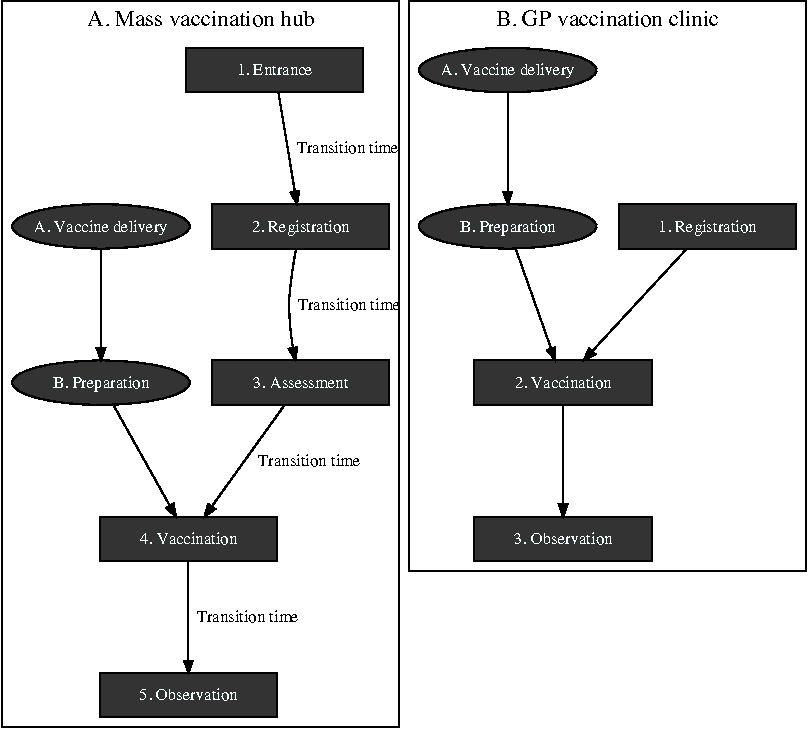
\includegraphics{Preprint_files/figure-latex/diagram-1} 

}

\caption{Queueing model for arena vaccination site (A) and GP vaccination site (B)}\label{fig:diagram}
\end{figure}

\hypertarget{queue-network-for-a-centralised-mass-vaccination-hub.}{%
\subsubsection{Queue network for a centralised mass vaccination
hub.}\label{queue-network-for-a-centralised-mass-vaccination-hub.}}

The proposed queue network for a mass vaccination hub is modelling on
the Pfizer vaccination hub based at the Royal Prince Albert (RPA)
hospital in Sydney. In this queue network, patients traverse five
stations: Entrance, Registration, Assessment, Vaccination and
Observation. The first four stations require the patient to wait for an
available staff member so these are modelled as queues, with new
arrivals serviced by the next available staff member on a
first-come-first-served basis. The observation stage does not require
patients to wait for an available staff member so this stage is modelled
as a stochastic waiting period, with longer waits for a small proportion
of individuals to reflect adverse reactions. Because mass vaccination
sites require a large premises, the queue network also incorporates a
short transition time between stations.

Vaccine doses must be prepared close to the time they are administered,
and clearly delays to this process would result in delays at the
vaccination stage. To capture this feature of the vaccination process,
the queue network includes a parallel queue for vaccine preparation (see
Figure \ref{fig:diagram}A) which merges with the patient queue at the
vaccination station. The distribution of vaccination tasks across these
stations is described in more detail below.

\hypertarget{entrance}{%
\paragraph{1. Entrance}\label{entrance}}

Patients arrive at the premises and queue up to get a temperature check
and to check in to the venue. Hand sanitiser and masks are made
available. This station would be overseen by one or more health staff
but could also be supplemented with volunteers to help marshal patients
to the next station.

\hypertarget{registration}{%
\paragraph{2. Registration}\label{registration}}

Having passed through the entrance station, patients join the queue for
registration. The registration desks are staffed by one or more
healthcare personnel. As part of the registration process, patients will
have their current appointment confirmed potentially could also book
their second vaccination. They are provided with pre-vaccination
information to read while they wait for the next station.

\hypertarget{assessment}{%
\paragraph{3. Assessment}\label{assessment}}

Once registered, patients join the queue for assessment. The purpose of
assessment is to make sure that the patient is clinically suitable to
receive the vaccine. During this stage the patients consent is also
recorded.

\hypertarget{vaccination}{%
\paragraph{4. Vaccination}\label{vaccination}}

Having been given final clearance to receive the vaccine at the
assessment station, patients join the queue for vaccination. Once a
vaccinator becomes available, the patient can take a seat and expose
their upper arm. The vaccinator confirms the patients name and details
then administers the vaccine. The vaccinator will apply a band-aid to
the vaccination site and note the vaccination time on a sticker and
apply this to the patients shoulder or lapel.

\hypertarget{observation}{%
\paragraph{5. Observation}\label{observation}}

Once vaccinated, patients advance to an observation area where they take
a seat and wait for the allotted time to ensure they experience no
adverse reaction. A staff member will advise the patient once their
allotted observation time has passed, at which point they can make their
way out of the premises.

\hypertarget{a.-vaccine-delivery}{%
\paragraph{A. Vaccine delivery}\label{a.-vaccine-delivery}}

The proposed queue network does not set out to model vaccine delivery.
All of our analyses assume that an adequate supply of vaccine doses is
available at the premises.

\hypertarget{b.-vaccine-preparation}{%
\paragraph{B. Vaccine preparation}\label{b.-vaccine-preparation}}

Vaccines are delivered in multi-dose vials containing 5-6 doses (Pfizer)
or 8-10 doses (AstraZeneca). The exact preparation steps will differ
depending on the vaccine being prepared. Steps incorporated at this
station may include logging the vial, visual inspection of the dose,
reconstitution (for the Pfizer vaccine), and drawing the vaccine into
syringes.

\hypertarget{queue-network-for-a-local-gp-vaccination-clinic}{%
\subsubsection{Queue network for a local GP vaccination
clinic}\label{queue-network-for-a-local-gp-vaccination-clinic}}

The proposed queue network for a local GP vaccination clinic is
presented in Figure \ref{fig:diagram}B. In this queue network, patients
traverse three distinct stations: Registration, Vaccination and
Observation. To advance to the Registration and Vaccination stations,
patients must wait for the next available staff member so these stations
are modelled as queueing processes, with patients serviced by the next
available staff member on a first-come-first-served basis. As with the
mass vaccination model, the observation station is modelled as a
stochastic waiting period rather than a queue, and there is a parallel
queue specified for vaccine preparation. The time taken to walk between
stations in a GP clinic is assumed to be negligible and not included in
the model. The distribution of vaccination tasks across these stations
is described in detail below.

\hypertarget{registration-1}{%
\paragraph{Registration}\label{registration-1}}

Patients arrive at the premises, and receive a temperature check on
entry. They are provided with pre-vaccination information and a
check-list of contra-indicated items, either as a paper form or on a
hand-held tablet. While seated in a waiting area, they read the provided
information and complete the pre-vaccination checklist. Once complete,
they return the paper form or tablet to the staff member and wait for
the next available vaccinator. This process is assumed to take place in
a shared waiting area, which may also be used for the observation step.

\hypertarget{vaccination-1}{%
\paragraph{Vaccination}\label{vaccination-1}}

Once a vaccinator becomes available, the patient advances to the
vaccination area, which may be a doctor's office or other suitable
cordoned-off area. The vaccinator reviews the patient's pre-vaccination
checklist, probes any items that have been checked and records the
patient's consent. The patient exposes their upper arm and the
vaccinator administers the vaccination and applies a band-aid to the
vaccination site. Finally the vaccinator notes the vaccination time on a
sticker and applies this to the patients shoulder or lapel.

\hypertarget{observation-1}{%
\paragraph{Observation}\label{observation-1}}

Once vaccinated, patients return to the waiting area where they take a
seat and wait for the allotted time to ensure they experience no adverse
reaction. The waiting area may be monitored by the same staff member who
is managing the registration process.

\hypertarget{assumed-service-times}{%
\subsection{Assumed service times}\label{assumed-service-times}}

For both the mass vaccination hub and GP vaccination clinic, the station
service times were modelled as exponential processes with fixed minimum
service times. The exception is the observation station, which was
modelled as bimodal distribution, with normally distributed observation
times for patients who did not experience an adverse reaction and
exponentially distributed observation times for a small random subset to
reflect a low incidence of adverse reactions. The assumed minimum
service times and exponential rate parameters for each station are
summarised in Table \ref{tab:serviceTimeAssumptions}), together with the
resulting distribution of service times.

\begin{table}[!h]

\caption{\label{tab:serviceTimeAssumptions}Service time parameter values and resulting distributions}
\resizebox{\linewidth}{!}{
\begin{tabular}[t]{>{\raggedright\arraybackslash}p{4cm}>{\raggedright\arraybackslash}p{2cm}>{\raggedright\arraybackslash}p{2cm}>{\raggedleft\arraybackslash}p{1cm}>{\raggedleft\arraybackslash}p{1cm}>{\raggedleft\arraybackslash}p{1cm}>{\raggedleft\arraybackslash}p{1cm}>{\raggedleft\arraybackslash}p{1cm}>{}l}
\toprule
\multicolumn{3}{c}{ } & \multicolumn{5}{c}{Percentiles} & \multicolumn{1}{c}{ } \\
\cmidrule(l{3pt}r{3pt}){4-8}
Station & Form & Formula & 5\% & 25\% & 50\% & 75\% & 95\% & Distribution\\
\midrule
\addlinespace[0.3em]
\multicolumn{9}{l}{\textbf{Arena model}}\\
\cellcolor{gray!6}{Preparation} & \cellcolor{gray!6}{exponential} & \cellcolor{gray!6}{1 + exp(3)} & \cellcolor{gray!6}{1.0} & \cellcolor{gray!6}{1.1} & \cellcolor{gray!6}{1.2} & \cellcolor{gray!6}{1.5} & \cellcolor{gray!6}{2.0} & \cellcolor{gray!6}{
\includegraphics[width=0.67in, height=0.17in]{Preprint_files/figure-latex//hist_21a334c96d80.pdf}}\\
Entrance & exponential & 2 + exp(1) & 2.1 & 2.3 & 2.7 & 3.4 & 5.0 & 
\includegraphics[width=0.67in, height=0.17in]{Preprint_files/figure-latex//hist_21a364609c41.pdf}\\
\cellcolor{gray!6}{Registration} & \cellcolor{gray!6}{exponential} & \cellcolor{gray!6}{3 + exp(0.7)} & \cellcolor{gray!6}{3.1} & \cellcolor{gray!6}{3.4} & \cellcolor{gray!6}{4.1} & \cellcolor{gray!6}{5.1} & \cellcolor{gray!6}{7.4} & \cellcolor{gray!6}{
\includegraphics[width=0.67in, height=0.17in]{Preprint_files/figure-latex//hist_21a31de3e677.pdf}}\\
Assessment & exponential & 2 + exp(1) & 2.0 & 2.3 & 2.7 & 3.4 & 5.0 & 
\includegraphics[width=0.67in, height=0.17in]{Preprint_files/figure-latex//hist_21a3612b6f9e.pdf}\\
\cellcolor{gray!6}{Vaccination} & \cellcolor{gray!6}{exponential} & \cellcolor{gray!6}{3 + exp(1)} & \cellcolor{gray!6}{3.1} & \cellcolor{gray!6}{3.3} & \cellcolor{gray!6}{3.7} & \cellcolor{gray!6}{4.5} & \cellcolor{gray!6}{6.2} & \cellcolor{gray!6}{
\includegraphics[width=0.67in, height=0.17in]{Preprint_files/figure-latex//hist_21a3c09ef0f.pdf}}\\
Observation & normal & norm(20, 0.5) & 19.8 & 19.9 & 20.0 & 20.1 & 20.2 & 
\includegraphics[width=0.67in, height=0.17in]{Preprint_files/figure-latex//hist_21a35da2d727.pdf}\\
\cellcolor{gray!6}{Adverse reaction} & \cellcolor{gray!6}{exponential} & \cellcolor{gray!6}{20 + exp(0.1)} & \cellcolor{gray!6}{20.4} & \cellcolor{gray!6}{22.7} & \cellcolor{gray!6}{26.9} & \cellcolor{gray!6}{34.3} & \cellcolor{gray!6}{50.1} & \cellcolor{gray!6}{
\includegraphics[width=0.67in, height=0.17in]{Preprint_files/figure-latex//hist_21a361f673f9.pdf}}\\
\addlinespace[0.3em]
\multicolumn{9}{l}{\textbf{GP model}}\\
Preparation & exponential & 1 + exp(2) & 1.0 & 1.1 & 1.3 & 1.7 & 2.5 & 
\includegraphics[width=0.67in, height=0.17in]{Preprint_files/figure-latex//hist_21a31e525b0e.pdf}\\
\cellcolor{gray!6}{Registration} & \cellcolor{gray!6}{exponential} & \cellcolor{gray!6}{1 + exp(3)} & \cellcolor{gray!6}{1.0} & \cellcolor{gray!6}{1.1} & \cellcolor{gray!6}{1.2} & \cellcolor{gray!6}{1.5} & \cellcolor{gray!6}{2.0} & \cellcolor{gray!6}{
\includegraphics[width=0.67in, height=0.17in]{Preprint_files/figure-latex//hist_21a335d9ef36.pdf}}\\
Vaccination & exponential & 1 + exp(3) & 1.0 & 1.1 & 1.2 & 1.5 & 2.0 & 
\includegraphics[width=0.67in, height=0.17in]{Preprint_files/figure-latex//hist_21a37095cce4.pdf}\\
\cellcolor{gray!6}{Observation} & \cellcolor{gray!6}{normal} & \cellcolor{gray!6}{norm(20, 0.5)} & \cellcolor{gray!6}{19.3} & \cellcolor{gray!6}{19.7} & \cellcolor{gray!6}{20.0} & \cellcolor{gray!6}{20.3} & \cellcolor{gray!6}{20.8} & \cellcolor{gray!6}{
\includegraphics[width=0.67in, height=0.17in]{Preprint_files/figure-latex//hist_21a32d8b28b.pdf}}\\
Adverse reaction & exponential & 20 + exp(0.1) & 20.5 & 23.0 & 27.0 & 33.9 & 49.5 & 
\includegraphics[width=0.67in, height=0.17in]{Preprint_files/figure-latex//hist_21a337056cc6.pdf}\\
\bottomrule
\end{tabular}}
\end{table}

\hypertarget{assumed-arrival-times}{%
\subsection{Assumed arrival times}\label{assumed-arrival-times}}

All models assumed patients were given fixed appointment slots across an
eight hour clinic running from 8am to 4pm. For mass vaccination hubs we
assumed that appointments would be given for quarter past the hour every
hour. For local GP hubs we assumed that appointments would be give in
ten minute intervals. Actual arrival times were based on the appointment
schedule but included some random noise, reflecting that most people
would turn up before their allotted time, while a smaller proportion
would arrive after their allotted time. Arrival times also accounted for
a small proportion of no-shows, set at 2\% for both local and mass
vaccination hubs. The actual number of arrivals per appointment interval
was calibrated to keep the queue performance metrics within reasonable
limits. As an example, Figure \ref{fig:arrivalTimes} presents simulated
arrival times for a mass vaccination hub at the rate of 120 arrivals
every hour, and a GP vaccination clinic at a rate of 4 arrivals every 10
minutes.

\begin{figure}

{\centering 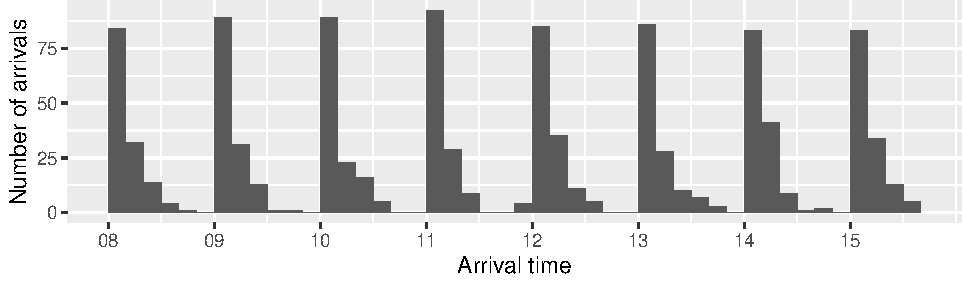
\includegraphics{Preprint_files/figure-latex/arrivalTimes-1} 

}

\caption{Randomly generated arrival times for a mass vaccination hub (A) and a GP vaccination clinic (B)}\label{fig:arrivalTimes}
\end{figure}

\hypertarget{staffing-levels}{%
\subsection{Staffing levels}\label{staffing-levels}}

For each of the proposed queue networks we specified models with
relatively low, medium and high staffing availability, ranging from 21
to 63 healthcare staff for mass vaccination sites and from 4 to 12
healthcare staff for GP vaccination clinics (Table \ref{tab:staffing}).
The distribution of staff across the queueing stations is kept stable
regardless of the total staffing capacity. For example, for the mass
vaccination model there are three staff assigned to the Registration
station for every one staff member assigned to the Preparation station,
regardless of the assumed size of the hub. This equivalence is
facilitates valid comparisons across hub sizes later in the analysis.

\begin{table}[!h]

\caption{\label{tab:staffing}Staff numbers by station for low, medium and high staffing availability}
\resizebox{\linewidth}{!}{
\begin{tabular}[t]{>{\raggedright\arraybackslash}p{2cm}>{\raggedleft\arraybackslash}p{2cm}>{\raggedleft\arraybackslash}p{2cm}>{\raggedleft\arraybackslash}p{2cm}>{\raggedleft\arraybackslash}p{2cm}>{\raggedleft\arraybackslash}p{2cm}>{\raggedleft\arraybackslash}p{2cm}}
\toprule
\multicolumn{1}{c}{ } & \multicolumn{6}{c}{Staff numbers} \\
\cmidrule(l{3pt}r{3pt}){2-7}
Size & Preparation & Entrance & Registration & Assessment & Vaccination & Total\\
\midrule
\addlinespace[0.3em]
\multicolumn{7}{l}{\textbf{Mass vaccination hub}}\\
\cellcolor{gray!6}{low} & \cellcolor{gray!6}{2} & \cellcolor{gray!6}{4} & \cellcolor{gray!6}{6} & \cellcolor{gray!6}{4} & \cellcolor{gray!6}{5} & \cellcolor{gray!6}{21}\\
medium & 4 & 8 & 12 & 8 & 10 & 42\\
\cellcolor{gray!6}{high} & \cellcolor{gray!6}{6} & \cellcolor{gray!6}{12} & \cellcolor{gray!6}{18} & \cellcolor{gray!6}{12} & \cellcolor{gray!6}{15} & \cellcolor{gray!6}{63}\\
\addlinespace[0.3em]
\multicolumn{7}{l}{\textbf{Local GP hub}}\\
low & 1 & * & 1 & * & 2 & 4\\
\cellcolor{gray!6}{medium} & \cellcolor{gray!6}{2} & \cellcolor{gray!6}{*} & \cellcolor{gray!6}{2} & \cellcolor{gray!6}{*} & \cellcolor{gray!6}{4} & \cellcolor{gray!6}{8}\\
high & 3 & * & 3 & * & 6 & 12\\
\bottomrule
\multicolumn{7}{l}{\rule{0pt}{1em}\textsuperscript{*} Not applicable}\\
\end{tabular}}
\end{table}

Note that the total staffing numbers given in Table \ref{tab:staffing}
only include staffing requirements for the stations in the assumed queue
network and do not cover all staffing needs to successfully run a
vaccination clinic. For example, the staff needed to oversee the
observation station are not included. Also not covered here are other
support staff, such as administrators, cleaners, marshals and caterers.
The number and type of support staff required will vary depending on the
size of the vaccination hub, and must also be taken into account when
planning vaccine distribution.

\hypertarget{queue-performance}{%
\subsection{Queue performance}\label{queue-performance}}

We use two metrics to quantify queue performance, total processing time
and staff utilisation. Total processing time, measured in minutes, is
the total time from start to finish of the queue network. Staff
utilisation is the average proportion of staff that are available across
the simulation run. An established property of queueing models is that
queue performance degrades when staff

\hypertarget{software-and-code}{%
\subsection{Software and code}\label{software-and-code}}

The analysis was performed using R version 4.0.3\textsuperscript{1} and
associated packages\textsuperscript{2}. Queueing models were simulated
using the \texttt{queuecomputer} package (ref). The complete source code
to reproduce this analysis can be accessed at
\url{https://github.com/CBDRH/}\ldots.

\hypertarget{results}{%
\section{Results}\label{results}}

\hypertarget{calibrating-arrivals-to-achieve-reasonable-service-times-and-staff-utilisation}{%
\subsection{Calibrating arrivals to achieve reasonable service times and
staff
utilisation}\label{calibrating-arrivals-to-achieve-reasonable-service-times-and-staff-utilisation}}

In this section we present estimates of average processing times and
average staff utilisation based on (i) the queue networks presented in
Figure \ref{fig: diagram} and (ii) the stochastic service times
described in Table \ref{tab:serviceTimeAssumptions}. The number of
available staff (and thus the number of open queues) at each station are
fixed to be constant at the levels set out in Table \ref{tab:staffing}.
Within each setting, the frequency of arrivals is increased gradually.
For example, for the mass vaccination site with low staffing numbers the
frequency of arrivals was increase from 10 per hour to 110 per hour, in
increments of 25. For each of the six implied models, the average
processing time and staff utilisation across 20 simulation runs are
presented in Figure \ref{fig:processingTimes} and
\ref{fig:staffUtilisation}.

\begin{figure}

{\centering 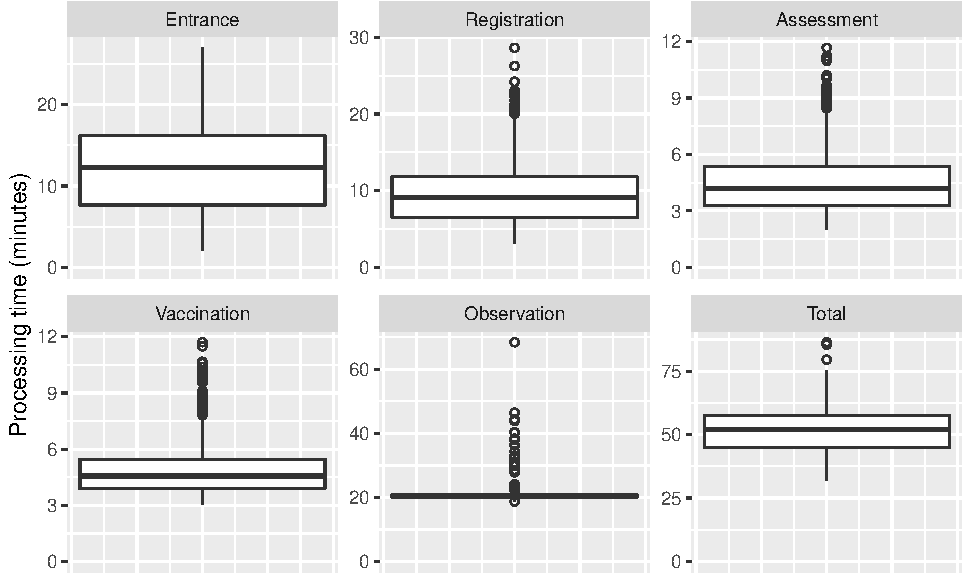
\includegraphics{Preprint_files/figure-latex/processingTimes-1} 

}

\caption{Average processing times by arrival frequency for a mass vaccination hub (A) and a GP vaccination clinic (B)}\label{fig:processingTimes}
\end{figure}

Figure \ref{fig:processingTimes} presents the average processing time as
the arrival frequency increases. When arrivals are set to their lowest
value, all processing times are within between 30 and 60 minutes (the
shaded band). In general, small increases to the average arrival rate
have a negligible impact on the overall processing time. However, once a
certain threshold is reached, the processing time quickly escalates. For
both mass vaccination hubs and GP vaccination clinics, the critical
threshold is lower in venues with relatively low staffing and higher in
venues with relatively high staffing, a point we will return to later.

Figure \ref{fig:staffUtilisation} presents the corresponding staff
utilisation for the Vaccination station, which was chosen as an example
because it is common to both the mass vaccination hub and the GP
vaccination clinic. Utilisation for the other stations are not presented
but display similar patterns.

\begin{figure}

{\centering 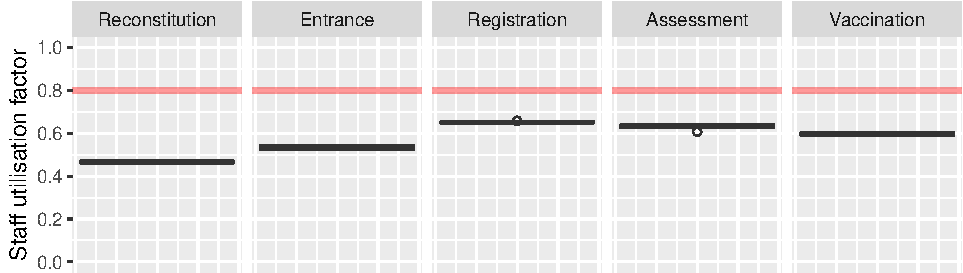
\includegraphics{Preprint_files/figure-latex/staffUtilisation-1} 

}

\caption{Average staff utilisation by arrival frequency for a mass vaccination hub (A) and a GP vaccination clinic (B)}\label{fig:staffUtilisation}
\end{figure}

As the arrival frequency increases, staff utilisation grows gradually.
The shaded area indicates a staff utilisation factor between 0.5 and
0.7. Beyond this level, utilisation rapidly increases as arrivals
increase.

These results emphasise the delicate balance between arrival frequency,
staff utilisation and processing times. If arrivals are two low,
processing times will be at an acceptable level but available the
available staff will be under-utilised. As arrivals increase, processing
times and staff utilisation increase accordingly, however if the rate of
arrivals grows too high staff utilisation passes a critical threshold
and processing times expand beyond reasonable levels.

Based on this calibration exercise, we specified the number of arrivals
such that the average processing times remained under an hour, and the
staff utilisation did not exceed 0.7 for any station. The resulting
arrival frequencies are presented in Table \ref{tab:arrivalFreq}.

\begin{table}[!h]

\caption{\label{tab:arrivalFreq}Arrival frequency by station for low, medium and high staffing availability}
\centering
\begin{tabular}[t]{>{\raggedright\arraybackslash}p{4cm}>{\raggedleft\arraybackslash}p{2cm}>{\raggedleft\arraybackslash}p{2cm}}
\toprule
Size & Appointment interval & Arrivals per interval\\
\midrule
\addlinespace[0.3em]
\multicolumn{3}{l}{\textbf{Mass vaccination hub}}\\
\cellcolor{gray!6}{low} & \cellcolor{gray!6}{60 minutes} & \cellcolor{gray!6}{60}\\
medium & 60 minutes & 120\\
\cellcolor{gray!6}{high} & \cellcolor{gray!6}{60 minutes} & \cellcolor{gray!6}{180}\\
\addlinespace[0.3em]
\multicolumn{3}{l}{\textbf{GP vaccination clinic}}\\
low & 10 minutes & 2\\
\cellcolor{gray!6}{medium} & \cellcolor{gray!6}{10 minutes} & \cellcolor{gray!6}{4}\\
high & 10 minutes & 6\\
\bottomrule
\end{tabular}
\end{table}

The chosen arrival frequencies were selected to increase linearly across
the low, medium and high staffing models: arrivals for the mass
vaccination hub were set at 60, 120 and 180 arrivals per hour at
relatively low, medium and high staffed hubs; arrivals for GP clinics
were set at 2, 4, and 6 arrivals per 10 minutes. Scaling the arrivals
and staffing in this way ensured that the baseline staff utilisation and
processing times remained constant across all models within the given
queue network (see Figure \ref{fig:baselineProcessingTimes} and Figure
\ref{fig:baselineUtilisation}). This equivalence facilitates comparisons
between hub sizes within the two queue networks.

\begin{figure}

{\centering 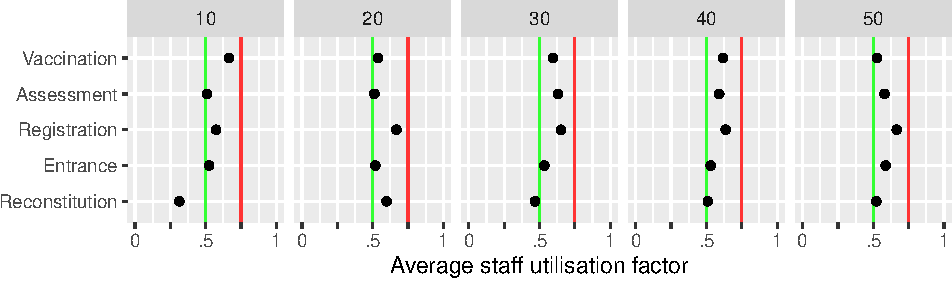
\includegraphics{Preprint_files/figure-latex/baselineUtilisation-1} 

}

\caption{Baseline staff utilisation factor for mass vaccination hubs (A) and GP vaccination clinics (B)}\label{fig:baselineUtilisation}
\end{figure}

The corresponding arrival frequencies are presented in Table
\ref{tab:arrivalFreqs}.

\begin{figure}

{\centering 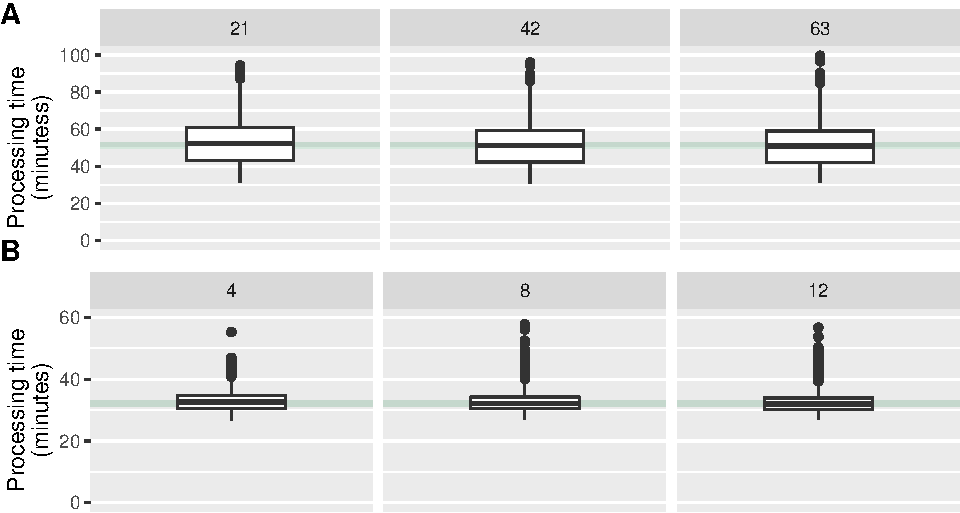
\includegraphics{Preprint_files/figure-latex/baselineProcessingTimes-1} 

}

\caption{Baseline processing times for the mass vaccination hub (A) and GP vaccination clinic (B)}\label{fig:baselineProcessingTimes}
\end{figure}

Te results in Figures \ref{fig:baselineProcessingTimes} and
\ref{fig:baselineUtilisation} illustrate that for both mass vaccination
hubs and GP clinics, the staff utilisation and processing times are
stable regardless of the staffing capacity. This equivalence is
important for the upcoming stress tests, because it means the different
models are starting from the same baseline in terms of queue
performance.

\hypertarget{daily-throughput}{%
\subsection{Daily throughput}\label{daily-throughput}}

Based on the calibrated baseline models, we can now estimate the number
of daily vaccinations possible at different site capacities while
maintaining processing times and staff utilisation within reasonable
limits. The results are presented in Figure
\ref{fig:baselineThroughput}.

\begin{figure}

{\centering 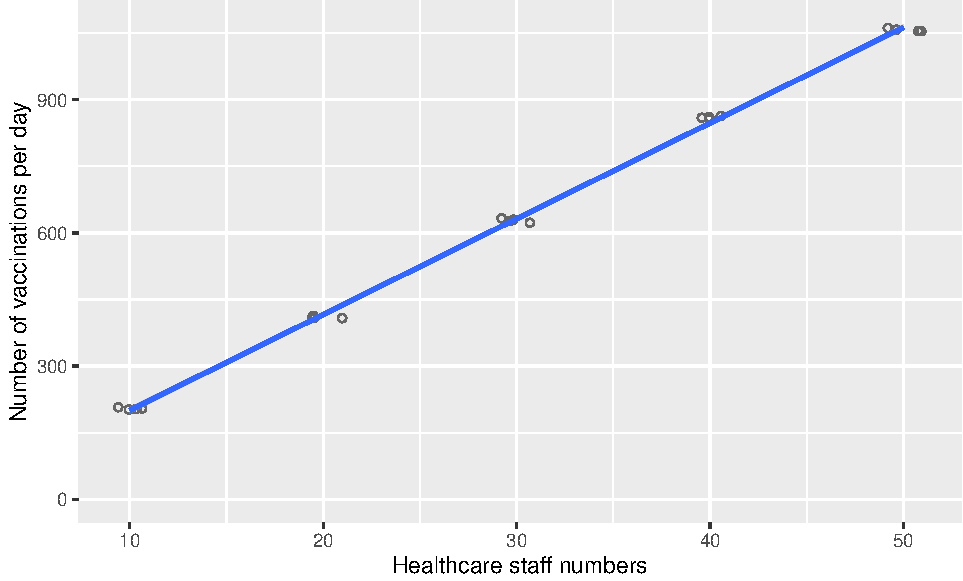
\includegraphics{Preprint_files/figure-latex/baselineThroughput-1} 

}

\caption{Baseline processing time for mass vaccination hubs (A) and GP vaccination clinics (B)}\label{fig:baselineThroughput}
\end{figure}

The results show that, while holding queue performance metrics constant,
the number of daily vaccinations scales linearly with increasing
healthcare staff for both the mass vaccination hub and GP vaccination
clinic. The potential throughput for an eight hour clinic at a mass
vaccination hubs, the daily throughput ranged from around 500 dose for a
relatively small hub to 1,400 vaccinations a day for a relatively hub.
For GP vaccination clinics, the estimated daily throughput ranged from
about 100 vaccinations a day for a relatively small practice to almost
300 a day for a relatively large practice.

\hypertarget{stress-tests}{%
\subsection{Stress tests}\label{stress-tests}}

In this section, we apply two stress tests to our baseline models. The
first test was to gradually increase arrivals which could reflect
efforts to increase throughput with the same staffing levels. This could
arise if the production of vaccine doses increased. The second stress
test was to gradually decrease staff numbers, which could reflect
inevitable fluctuations in staff availability due to illness etc, or
healthcare staff having to attend to a medical emergency.

\hypertarget{increasing-arrivals}{%
\subsubsection{Increasing arrivals}\label{increasing-arrivals}}

Figure \ref{fig:processingTimeTest} presents the average processing time
based on incrementing the arrival frequency from the levels set for the
baseline models. For mass vaccination hubs and GP clinics, increasing
the number of arrivals results in increased processing times. However,
the rate of increase in processing times is larger for sites with
relatively low healthcare staff compared to sites with relatively high
healthcare staffing.

\begin{figure}

{\centering 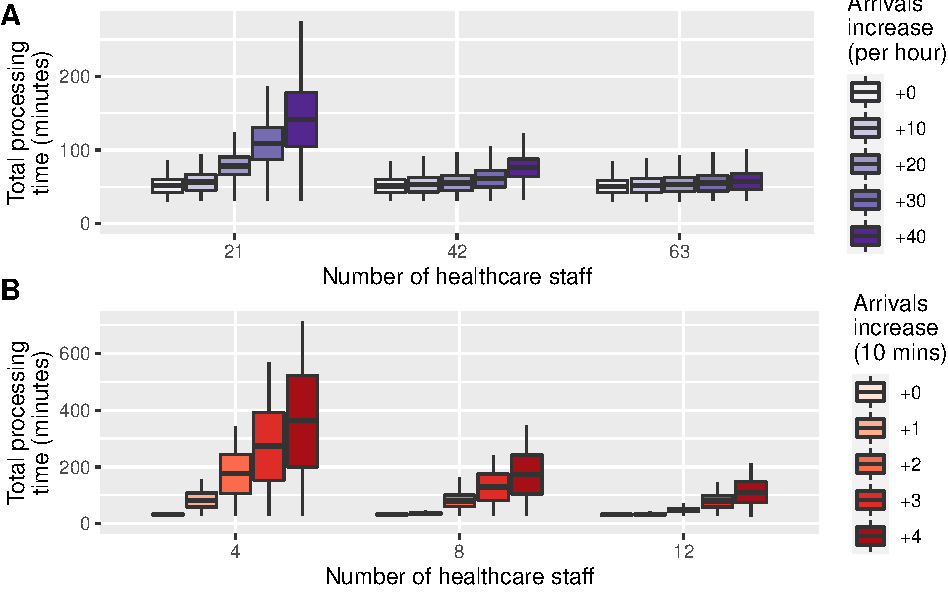
\includegraphics{Preprint_files/figure-latex/processingTimeTest-1} 

}

\caption{Increase in processing time with increased arrivals by site size for mass vaccination hubs (A) and GP vaccination clinics (B)}\label{fig:processingTimeTest}
\end{figure}

\begin{figure}

{\centering 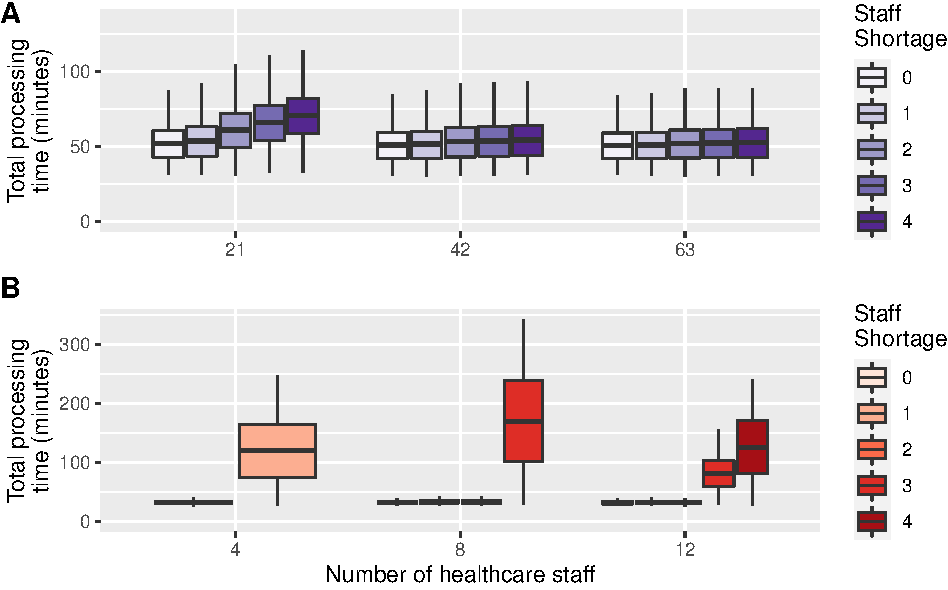
\includegraphics{Preprint_files/figure-latex/staffShortageTest-1} 

}

\caption{Increase in processing time with staff shortages by site size}\label{fig:staffShortageTest}
\end{figure}

\hypertarget{staff-shortages}{%
\subsubsection{Staff shortages}\label{staff-shortages}}

Figure \ref{fig:staffShortageTest} presents the average processing time
based on gradually decreasing the available staff for a given model.
These results show that---unsurprisingly---small vaccination sites with
limited staff numbers are quickly affected by staff shortages, whereas
large vaccination hubs with more staff can still maintain queue
performance with the same number of staff shortages.

\hypertarget{discussion}{%
\section{Discussion}\label{discussion}}

\hypertarget{summary-and-discussion-of-main-results}{%
\subsection{Summary and discussion of main
results}\label{summary-and-discussion-of-main-results}}

We have used queueing simulation methods to model the vaccination
process based on two delivery approaches: a large mass vaccination hub
and a small GP vaccination clinic. For each site, we calibrated the
number of arrivals that could be vaccinated over an eight hour period
while keeping two queue performance measures---staff utilisation and
total processing time---constrained to reasonable levels. Our results
provide estimates of potential daily throughput for these distinct
vaccine delivery models across a range of staffing levels. Under our
assumed service times, a relatively small GP clinic could perform around
100 vaccinations over an eight-hour clinic, while a relatively large
mass vaccination hub could perform around 1,400 vaccinations over the
same time period. Put differently, one large mass vaccination hub can
achieve the same coverage as 14 GP small vaccination clinics.

These throughput estimates have reasonable face-validity. The mass
vaccination hub trialled by NSW Health in a 2008 pandemic response
planning exercise administered 498 vaccines in five hours using a queue
network similar to our model delivered through a local school. The RPA
Pfizer clinic has been delivering between 1,100 and 1,400 vaccinations
per day throughout March.

Our models suggest that daily vaccination capacity scales linearly with
staffing capacity while maintaining a constant queue performance.
However, there are several other facets of the vaccine delivery process
that are likely to offer economies of scale. For example, given the low
incidence of adverse events, a high-capacity post vaccination area
observation area could be overseen by a single staff member. Economies
of scale area also likely for vaccine delivery as it may be more
efficient and cost effective to coordinate a single delivery to one
centralised hub rather than multiple deliveries to numerous smaller
clinics.

By stressing our baseline models, we have shown that mass vaccination
hubs are better placed to scale up daily throughput without increasing
staff numbers and maintaining acceptable queue performance. Mass
vaccination hubs are also are more resilient to staff shortages.

\hypertarget{policy-implications}{%
\subsection{Policy implications}\label{policy-implications}}

To date, the Australian Government's approach to vaccine delivery has
relied on hospital hubs to administer the Pfizer Vaccine to the highest
priority phase, whereas delivery of subsequent phases is planned through
smaller sites, including general practices, Aboriginal Controlled
Community Health Services, and community pharmacies to administer the
AstraZeneca vaccine to the bulk of the Australian population. There has
been little emphasis on the use of mass vaccination hubs to be included
in vaccination efforts, although previous pandemic planning exercises
found this model to be effective, and it has been applied successfully
in Australia (during the first vaccine phase) and overseas (ref to UK).

{[}Other key points to be added{]}

\hypertarget{limitations}{%
\subsection{Limitations}\label{limitations}}

Our analysis does not account for essential staff who are not involved
in the queueing process but do need to be considered when estimating
staff requirements. Our models assume sufficiently available vaccine
doses, and do not address the challenges of vaccine procurement or the
logistics of delivering vaccine doses to the venues where they will of
administered. The assumed queue networks rely on subjective assumptions
of the distribution of service times at each station. We specified
service times that had reasonable face-validity and produced realistic
estimates of overall processing times. This could be improved in the
future through a time-use survey to empirically estimate service time
distributions for each station in a queue network.

\hypertarget{conclusion}{%
\subsection{Conclusion}\label{conclusion}}

Stochastic queueing models can be used to simulate vaccination queues,
estimate daily throughput based on given staff availability and inform
service delivery. Different models of vaccine distribution have
different benefits and challenges. Mass vaccination clinics offer a
higher daily throughput and are more resilient to increased arrivals and
decreased staff availability, however they require larger premises and
higher staffing numbers. GP vaccination clinics can perform vaccinations
at a similar rate per staff member compared to mass vaccination hubs,
however it may be difficult to sustain a high throughput given existing
workloads. A diverse profile of vaccination sites, drawing on the
benefits of both distribution models, may help to maximise the daily
vaccination rate and vaccinate the Australian population against
COVID-19 as quickly as possible.

\hypertarget{contributions}{%
\section{Contributions}\label{contributions}}

\hypertarget{acknowledgements}{%
\section{Acknowledgements}\label{acknowledgements}}

This research was supported by the generous assistance of Ian Sharp,
philanthropic supporter of UNSW research, and by a research seed grant
provided by the Sydney Partnership for Health, Education, Research and
Enterprise (SPHERE) Infectious diseases, Immunity and Inflammation
(Triple-I) Clinical Academic Group.

\newpage

\hypertarget{references}{%
\section*{References}\label{references}}
\addcontentsline{toc}{section}{References}

\hypertarget{refs}{}
\begin{CSLReferences}{0}{0}
\leavevmode\hypertarget{ref-R-base}{}%
\CSLLeftMargin{1. }
\CSLRightInline{R Core Team. \emph{R: A Language and Environment for
Statistical Computing}. R Foundation for Statistical Computing; 2019.
\url{https://www.R-project.org/}}

\leavevmode\hypertarget{ref-tidyverse2019}{}%
\CSLLeftMargin{2. }
\CSLRightInline{Wickham H, Averick M, Bryan J, et al. Welcome to the
{tidyverse}. \emph{Journal of Open Source Software}. 2019;4(43):1686.
doi:\href{https://doi.org/10.21105/joss.01686}{10.21105/joss.01686}}

\end{CSLReferences}

\bibliographystyle{unsrt}
\bibliography{packages.bibreferences.bib}


\end{document}
